\documentclass[crop,tikz,11pt]{standalone}
\usepackage{geometricfigures}
\usepackage{amsmath,amssymb}
\usepackage{pgfplots}
\pgfplotsset{compat=1.18}
\usetikzlibrary{arrows.meta,decorations.markings,patterns,intersections}
\usepgfplotslibrary{fillbetween}

\definecolor{lib}{HTML}{3B75AF}
\definecolor{rot}{HTML}{C1701E}
\definecolor{sep}{HTML}{B03030}
\definecolor{net}{HTML}{4E9A4E}

\begin{document}
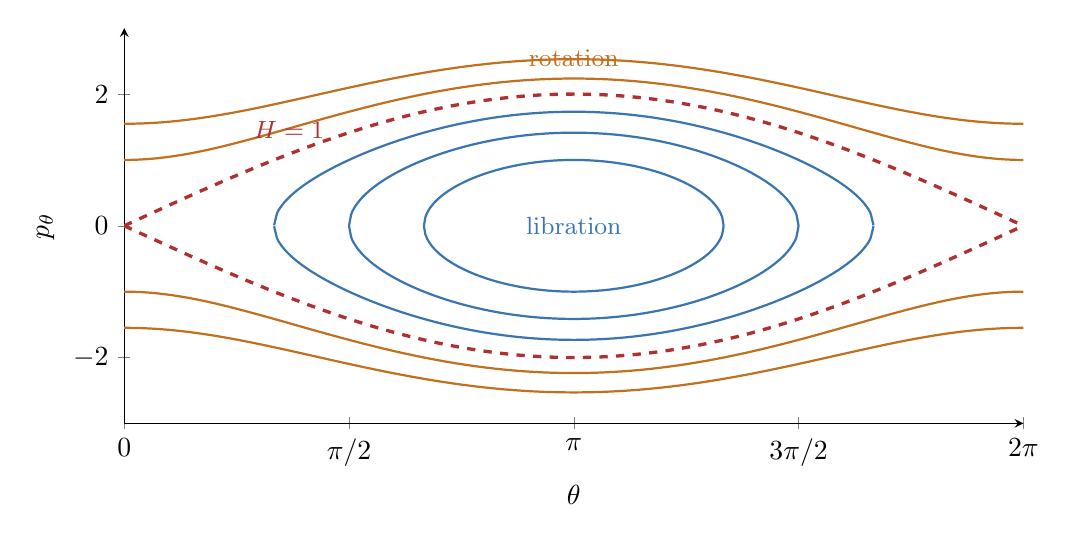
\begin{tikzpicture}
\begin{axis}[width=13cm,height=6.6cm,xmin=0,xmax=6.2832,ymin=-3,ymax=3,
  xtick={0,1.5708,3.1416,4.7124,6.2832},
  xticklabels={$0$,$\pi/2$,$\pi$,$3\pi/2$,$2\pi$},
  xlabel={$\theta$},ylabel={$p_\theta$},
  axis lines=left,every axis plot/.append style={smooth,samples=200}]
  % Librating level sets. Each one is drawn only between its own turning points
  % theta = arccos(H) and 2pi - arccos(H), which is where p_theta = 0 and the
  % loop closes. The domain has to be cut per level: outside it 2(H - cos theta)
  % is negative, the max(0,.) that keeps the sqrt real returns zero, and the plot
  % runs on along p_theta = 0 -- three levels' worth of that is a spurious
  % horizontal line across the whole portrait. The max(0,.) stays for roundoff at
  % the two endpoints; it is the domain, not the clamp, that does the work.
  \foreach \H/\ta/\tb in {-0.5/2.0944/4.1888, 0/1.5708/4.7124, 0.5/1.0472/5.2360}{
    \addplot[lib,thick,domain=\ta:\tb]{ sqrt(max(0,2*(\H-cos(deg(x)))))};
    \addplot[lib,thick,domain=\ta:\tb]{-sqrt(max(0,2*(\H-cos(deg(x)))))};
  }
  % separatrix
  \addplot[sep,very thick,dashed,domain=0:6.2832]{ 2*abs(sin(deg(x/2)))};
  \addplot[sep,very thick,dashed,domain=0:6.2832]{-2*abs(sin(deg(x/2)))};
  % rotating
  \foreach \H in {1.5,2.2}{
    \addplot[rot,thick,domain=0:6.2832]{ sqrt(2*(\H-cos(deg(x))))};
    \addplot[rot,thick,domain=0:6.2832]{-sqrt(2*(\H-cos(deg(x))))};
  }
  \node[lib] at (axis cs:3.1416,0.0) {\small libration};
  \node[rot] at (axis cs:3.1416,2.55) {\small rotation};
  \node[sep] at (axis cs:1.15,1.45) {\small $H=1$};
\end{axis}
\end{tikzpicture}
\end{document}
